\documentclass{article}

\usepackage{fancyhdr}
\usepackage{extramarks}
\renewcommand{\thispagestyle}[1]{} % damit Titelseite Kopfzeile bekommt
\usepackage{amsmath}
\usepackage{amsthm}
\usepackage{amsfonts}
\usepackage{tikz}
\usepackage[plain]{algorithm}
\usepackage{algpseudocode}
\usepackage{listings}
\lstset{language=C++, numbers=left, frame=single,}
\usepackage[utf8]{inputenc}
\usepackage{paralist}
\usepackage{tikz}
\usepackage{multicol}

\usetikzlibrary{automata,positioning}

%
% Basic Document Settings
%

\topmargin=-0.45in
\evensidemargin=0in
\oddsidemargin=0in
\textwidth=6.5in
\textheight=9.0in
\headsep=0.25in

\linespread{1.1}

\pagestyle{fancy}
\lhead{\hmwkGroup\\\hmwkTitle}
\rhead{\hmwkAuthorName}
\lfoot{\lastxmark}
\cfoot{\thepage}

\renewcommand\headrulewidth{0.4pt}
\renewcommand\footrulewidth{0.4pt}

\setlength\parindent{0pt}

%
% Create Problem Sections
%

\newcommand{\enterProblemHeader}[1]{
    \nobreak\extramarks{}{Aufgabe \arabic{#1} wird auf nächster Seite fortgesetzt\ldots}\nobreak{}
    \nobreak\extramarks{Aufgabe \arabic{#1} (fortgesetzt)}{Aufgabe \arabic{#1} wird auf nächster Seite fortgesetzt\ldots}\nobreak{}
}

\newcommand{\exitProblemHeader}[1]{
    \nobreak\extramarks{Aufgabe \arabic{#1} (fortgesetzt)}{Aufgabe \arabic{#1} wird auf nächster Seite fortgesetzt\ldots}\nobreak{}
    \stepcounter{#1}
    \nobreak\extramarks{Aufgabe \arabic{#1}}{}\nobreak{}
}

\setcounter{secnumdepth}{0}
\newcounter{partCounter}
\newcounter{homeworkProblemCounter}
\setcounter{homeworkProblemCounter}{1}
\nobreak\extramarks{Aufgabe \arabic{homeworkProblemCounter}}{}\nobreak{}

%
% Homework Problem Environment
%
% This environment takes an optional argument. When given, it will adjust the
% problem counter. This is useful for when the problems given for your
% assignment aren't sequential. See the last 3 problems of this template for an
% example.
%

\newenvironment{homeworkProblem}[1][-1]{
    \ifnum#1>0
        \setcounter{homeworkProblemCounter}{#1}
    \fi
    \section{Aufgabe \arabic{homeworkProblemCounter}}
    \setcounter{partCounter}{1}
    \enterProblemHeader{homeworkProblemCounter}
}{
    \exitProblemHeader{homeworkProblemCounter}
}

%
% Homework Details
%   - Title
%   - Due date
%   - Class
%   - Section/Time
%   - Instructor
%   - Author
%

\date{27.4.2018}
\newcommand{\hmwkTitle}{Übungsblatt\ \#3}
\newcommand{\hmwkGroup}{Übungsgruppe 16}
\newcommand{\hmwkDueDate}{3. Mai 2018}
\newcommand{\hmwkClass}{Datenstrukturen und Algorithmen}
\newcommand{\hmwkAuthorName}{\textbf{Finn Hess (378104), Jan Knichel (377779), Paul Orschau (381085)}}

%
% Title Page
%

\title{
    \vspace{2in}
    \textmd{\textbf{\hmwkClass:\ \hmwkTitle}}\\
    \normalsize\vspace{0.1in}\small{Abgabe\ am\ \hmwkDueDate\ }\\
    \vspace{3in}
}

\author{\hmwkAuthorName}

\renewcommand{\part}[1]{\textbf{\large Part \Alph{partCounter}}\stepcounter{partCounter}\\}

%
% Various Helper Commands
%

% Useful for algorithms
\newcommand{\alg}[1]{\textsc{\bfseries \footnotesize #1}}

% For derivatives
\newcommand{\deriv}[1]{\frac{\mathrm{d}}{\mathrm{d}x} (#1)}

% For partial derivatives
\newcommand{\pderiv}[2]{\frac{\partial}{\partial #1} (#2)}

% Integral dx
\newcommand{\dx}{\mathrm{d}x}

% Alias for the Solution section header
\newcommand{\loesung}{\textbf{\large Lösung}}

% Parts
\newcommand{\teil}[1]{\vspace{15pt}\textbf{Teil #1}}


%
% Start of Document
%

\begin{document}

  \maketitle

  \pagebreak

  \begin{homeworkProblem}
    
    \teil{a)}
    
    Notation: Sei $N_h$ die Anzahl innerer Knoten eines Baumes der Höhe $h$.
    
    Sei Aussage $A(h)$ gegeben durch $N_h \leq 2^h-1$ (Der Baum hat höchstens $2^h-1$ innere Knoten).
    
    \vspace{5pt}
    Beweis der Aussage $A(h)$ per Induktion nach $h \in \mathbb N$:
          
    \vspace{5pt}
    Induktionsanfang: $h_0=0$
    
    $A(0):$ Der Baum besteht nur aus der Wurzel, es gilt also $N_0=0 \leq 0=2^0-1$. \checkmark
    
    \vspace{5pt}
    Induktionsvoraussetzung: Sei $h\in\mathbb N$ fest, aber beliebig, und es gelte $A(h)$.
    
    \vspace{5pt}
    Induktionsschritt: $h\rightarrow h+1$
    
    $A(h+1): N_{h+1}
    \stackrel{*}{\leq}      N_h + 2^h
    \stackrel{(I.V.)}{\leq} 2^h - 1 + 2^h 
    = 2^h(1+1)-1 = 2^{h+1}-1 $ \checkmark \qed
    
    \vspace{5pt}
    *Der Baum der Höhe $h$ kann höchstens $2^h$ Blätter haben, die zu inneren Knoten des Baums der Höhe $h+1$ werden können. Daher gilt diese Ungleichung.
              
    \teil{b)}
    
    Preorder Linearisierung: 1 2 3
    
    Postorder Linearisierung: 3 2 1
    
    Zwei Bäume:
    
    \begin{multicols}{2}
        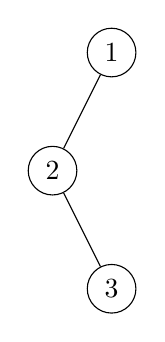
\begin{tikzpicture}
        \node[circle,draw](z){1}
          child{
            node[circle,draw]{2} child[missing] child{node[circle,draw] {3}}}
          child[missing]{};
        \end{tikzpicture}

        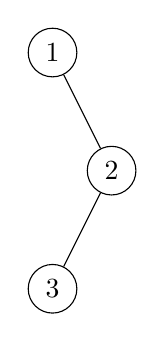
\begin{tikzpicture}
        \node[circle,draw](z){1}
          child[missing]{}
          child{
            node[circle,draw]{2} child{node[circle,draw] {3}} child[missing] };
        \end{tikzpicture}
    \end{multicols}
    
    $\Rightarrow$ Nicht eindeutig!

    \pagebreak   
    
    \teil{c)}
    
    Falls Mirror- und Inorder-Linearisierung eines Baumes gegeben sind, ist der Baum eindeutig bestimmt.
    
    \vspace{10pt}
    Beweis (konstruktiv):
    
    Sei die Mirror-Linearisierung gegeben durch $M_1, M_2, \dots, M_n$
    
    und die Inorder-Linearisierung durch $I_1, I_2, \dots, I_n$.
    
    In der Mirror-Linearisierung tritt die Wurzel des Baumes stets als erstes auf, die Wurzel des Baumes ist stets $M_1$. Nun unterteilt dann die Inorder-Linearisierung in zwei Hälften:
    
    $L_1, L_2, \dots, L_{k-1}, M_1, L_{k+1}, \dots, L_{n-1}, L_n$ 
    
    Da es die Inoder-Linearisierung ist, gehören nun $L_1, \dots, L_{k-1}$ zum \textbf{linken} Teilbaum und $L_{k+1}, \dots, L_n$ zum \textbf{rechten} Teilbaum. Sollte es eine der beiden Knotensammlungen nicht geben, zum Beispiel weil $M_1$ an erster oder letzter Stelle auftritt, gibt es den jeweiligen Teilbaum einfach nicht.
    
    Nun durchsucht man $M_2, \dots, M_n$ nach dem ersten Element, welches auch in $L_1, \dots, L_{k-1}$ vorkommt, also dem ersten Element, welches zum linken und nicht zum rechten Teilbaum gehört. Wir nennen dieses Element für den Moment $X$.
    
    Nun ist gerade $M_2, \dots$ bis (nicht einschließlich) $X$ die Preorder-Linearisierung des rechten Teilbaumes! Damit ist der rechte Teilbaum der Wurzel eindeutig bestimmt, denn wir kennen sowohl seine Inorder- als auch seine Preorder-Linearisierung.
    
    Nun ist $X$ die Wurzel des linken Teilbaums, die verbleibenden Elemente der Mirror-Linearisierung dessen Mirror-Linearisierung und $L_1, L_2, \dots$ bis (nicht einschließlich) $M_1$ dessen Inorder-Linearisierung. Nun kann man das Verfahren also von vorne beginnen, so lange bis keine Knoten mehr übrig sind und der Baum vollständig ist.

  \end{homeworkProblem}

  \begin{homeworkProblem}
    
    \texttt{traverse(G)} besucht jeden Knoten \textbf{mindestens} einmal, da jeder Knoten (außer der Wurzel) nach Eigenschaft 2 einen "Vorgängerknoten" besitzt, welcher die Funktion \texttt{visit(v)} auf ihm ausführen wird. Die Wurzel wird auch besucht, denn mit ihr startet die Rekursion in Zeile 8.
  
    Jeder Knoten wird also mindestens einmal besucht, gibt sich aber \textbf{höchstens} einmal aus, da jeder Knoten sich "merkt", falls er schonmal besucht worden ist, und bei eventuellen weiteren Besuchen einfach gar nichts tut.
    
    Damit wird jeder Knoten von \texttt{traverse(G)} also \textbf{genau einmal} ausgegeben!
    
  \end{homeworkProblem}

  \pagebreak

  \begin{homeworkProblem}

    \teil{a)}
    
    Implementiert man die Liste mit zwei Zeigern, welche auf Anfang und Ende der Liste zeigen (bspw. doppelt verkettete Liste), so sind alle 5 Operationen in konstanter Zeit ausführbar.
    
    Für \texttt{isEmpty} braucht man nur zu prüfen, ob beide Zeiger auf \texttt{Null} zeigen. Dafür spielt die Eingabelänge keine Rolle.
    
    Für \texttt{enqueueFront} und \texttt{enqueueBack} fügt man einfach ein Element am Anfang/Ende der Liste hinzu und verschiebt den Zeiger. Die Dauer hängt ebenfalls nicht von der Eingabelänge ab.
    
    Für \texttt{dequeueFront} und \texttt{dequeueBack} entfernt man das Element, auf welches der jeweilige Zeiger zeigt, und verschiebt den Zeiger danach. Sollte nur ein Element in der Liste sein, d.h. wenn nach der Operation die Liste leer ist, muss man zusätzlich noch beide Zeiger auf Null setzen. Die Dauer hängt wieder nicht von der Eingabelänge ab.
    
    \teil{b)}

    Es ist unmöglich, die Operationen in $\mathcal O(1)$ auszuführen, denn wenn man z.B. mit \texttt{enqueueFront} ein Element am Anfang der Liste einfügen möchte, müssen alle Elemente um 1 nach hinten verschoben werden, was nur in $\mathcal O(n)$ möglich ist, da es von der Länge der Liste abhängen muss. Das selbe gilt für das Entfernen eines Elements mit \texttt{dequeueFront}.
    
    \teil{c)}
    
    \begin{itemize}
      \item \texttt{add} kann in $\mathcal O(n)$ ausgeführt werden, denn man muss das Element, welches hinzugefügt werden soll, im schlimmsten Fall mit allen bereits in $s$ enthaltenen Elementen vergleichen, benötigt also höchstens $n$ Vergleiche. 

      \item \texttt{contains} kann in $\mathcal O(n)$ ausgeführt werden, denn um das gesuchte Element zu finden, muss man im schlimmsten Fall alle bereits in $s$ enthaltenen Elemente überprüfen, benötigt also höchstens $n$ Vergleiche.

      \item \texttt{union} kann nur in $\mathcal O(n)$ ausgeführt werden, falls die Sets (vielleicht mittels Hashwerten) so implementiert sind, dass \texttt{contains} in $\mathcal O(1)$ liegt. Dann erstellt man die Vereinigung von $s1$ und $s2$ indem man zunächst $s1$ kopiert und dann für jedes Element von $s2$ überprüft, ob es schon in $s1$ erhalten war. War es nicht enthalten, fügt man es zur Vereinigung hinzu. Da man also höchstens $n$-mal \texttt{contains} aufrufen muss (falls $s1$ keine Elemente enthält, also alle $n$ Elemente in $s1$ sind), liegt die Laufzeit von \texttt{union} in $\mathcal O(n)$.
    \end{itemize}

    \teil{d)}
    
    Eine solche Implemetierung gibt es nicht, da die Erstellung des Ausgabesets auf jeden Fall von der Größe der beiden Eingabesets abhängen muss. Eine Vereinigung von zwei Sets mit jeweils einem Element braucht weniger Zeit zum Beschreiben des Speichers, Kopieren der Daten, etc. als eine Vereinigung von zwei Sets mit jeweils 1 Mio. Elementen.

  \end{homeworkProblem}

  \pagebreak

  \begin{homeworkProblem}
    
    \teil{a)}
    
    $S(n) \in \mathcal O(1)$, wenn die doppelten Elemente direkt am Anfang der Liste stehen, da dann nur das erste Element abgespeichert wird, weil danach der Algorythmus abbricht.

    $S(n) \in \Omega(n-1)$, wenn das doppelte Element am Ende der Liste steht, da dann die gesamte Liste bis auf das letzte (doppelte) Element abgespeichert wird.

    \teil{b)}

    Der Best Case ist 2, wenn die beiden 1er direkt am Anfang der Liste stehen, denn dann braucht der Algorithmus eine Zeiteinheit für die erste 1 und eine für die zweite und bricht danach ab, weil das doppelte Element bereits gefunden ist.

    Der Worst Case ist n, wenn die zweite 1 an der letzten Stelle der Liste steht, da dann der Algorithmus jedes einzelne Element überprüfen muss, bis er am Ende das doppelte gefunden hat und dann abbricht.
    Der Average Case ist die Summe aller Wahrscheinlichkeiten, dass die zweite 1 an der Stelle i liegt multipliziert mit der entsprechenden Laufzeit:
    \begin{equation}
      \begin{split}
        A(n) & = \frac{\sum\limits_{i=2}^n Anz\text{\{Eingaben mit zweiter 1 bei i\}} * t\text{\{Zweite 1 an der Stelle i\}}}{D_n} \\
        & = \frac{\sum\limits_{i=2}^n (i-1)(n-2)! * i}{\frac{n!}{2}} \\
        & = \frac{2(n-2)!}{n!} \sum\limits_{i=2}^n (i-1) * i \\
        & = \frac{2(n-2)!}{n!} \sum\limits_{i=2}^n [i^2-i] \\
        & = \frac{2(n-2)!}{n!} [\sum\limits_{i=2}^ni^2 -\sum\limits_{i=2}^n i] \\
        & = \frac{2(n-2)!}{n!} [\frac{n(n+1)(2n+1)}{6}-1 -\frac{3n(n+1)}{6}+1] \\
        & = \frac{2(n-2)!}{n!} * \frac{n(n+1)(2n+1)-3n(n+1)}{6} \\
        & = \frac{2(n-2)!}{n!} * \frac{2n^3 + 3n^2 + n - (3n^2 + 3n)}{6} \\
        & = \frac{2(n-2)!}{n!} * \frac{2n^3 - 2n}{6} \\
        & = \frac{2(n-2)!}{n!} * \frac{n^3 - n}{3} \\
        & = \frac{2(n-2)!}{n!} * \frac{(n-1)n(n+1)}{3} \\
        & = \frac {2}{3} * (n+1)
      \end{split}
    \end{equation}

    \pagebreak
    
    \teil{c)}

    \lstinputlisting{Code/4_c.cpp}
    
    Der Algorithmus hat offensichtlich konstanten Speicherbedarf,
    
    denn unabhängig von der Eingabelänge braucht er immer nur i und j als Variablen.
    
    Die Worst-Case Laufzeit ist in $\mathcal O(n^2)$, denn die äußere Schleife läuft $(n-1)$-mal, die innere Schleife macht immer $(n-i)$ Vergleiche.
    
    \begin{equation}
      W(n) = \sum\limits_{i=1}^{n-1} (n-i) = \sum\limits_{i=1}^{n-1} i = \frac{n(n-1)}{2}
      = \frac{n^2-n}{2} \in \mathcal O(n^2)
    \end{equation}
    
  \end{homeworkProblem}
  
  \teil{d)}
  
  \lstinputlisting{Code/4_d.cpp}
  
  Der Algorithmus hat eine lineare Laufzeit, denn er hat keine verschachtelten \texttt{for}-Loops. Je nachdem, welche Zeilen also eine Zeiteinheit benötigen, beträgt die Laufzeit zum Beispiel $2n$.

\end{document}